\usetikzlibrary{calc}
\tikzset{
	sqrwave/.pic={
			\draw (0,0) -- (0,.5) -- (${#1}*(1,0)+(0,.5)$) --
			(${#1}*(1,0)+(0,0)$) -- (1,0);
	}
}
\tikzset{
	sinewave/.pic={
		\draw (0,0) sin (.25,#1) cos (.5,0) sin (.75,-#1) cos (1,0);
	}
}
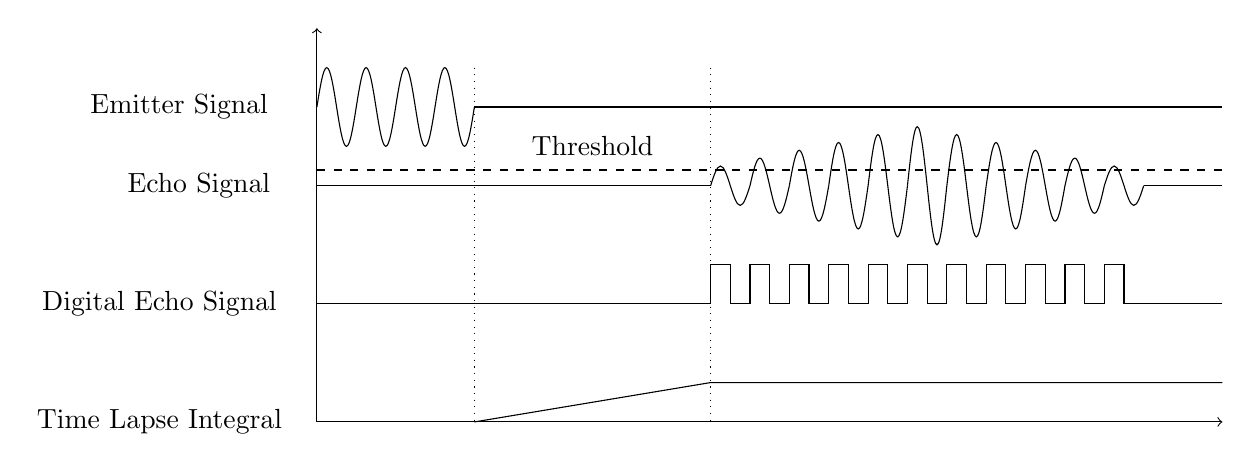
\begin{tikzpicture}
%axis
\draw[<->] (0,5) -- (0,0) -- (11.5,0);

%emitter signal 
\node at (-1.75,4) {Emitter Signal};
\begin{scope}[shift={(0,4)}]
	\foreach \x in{0,1,...,3}
	{
		\draw pic[x={(.5,0)},shift={(\x,0)}] {sinewave=.5};
	}
	\draw (2,0) -- (11.5,0);
\end{scope}

% receive signal
\node at (-1.5,3) {Echo Signal};
\node at (-2,1.5) {Digital Echo Signal};
\begin{scope}[shift={(0,2)}]
	% signal
	\begin{scope}[shift={(5,0)}]
		\foreach \x [evaluate=\x as \xval using 1.5-(((\x-5)/5)^2)^(1/2)] in
		{0,1,...,10}
		{
			\draw pic[x={(.5,0)},shift={(\x,-.5)}] {sqrwave=.5};
			\draw pic[x={(.5,0)},y={(0,.5)},shift={(\x,2)}] {sinewave=\xval};
		}
	\end{scope}
	%threshold line
	\node at (3.5,1.5) {Threshold};
	\draw[dashed] (0,1.2) -- (11.5,1.2);

	% axis
	\draw (0,1) -- (5,1);
	\draw (10.5,1) -- (11.5,1);

	\draw (0,-.5) -- (5,-.5);
	\draw (10.5,-.5) -- (11.5,-.5);
\end{scope}

%time lapse
% vertical dividers
\node at (-2,0) {Time Lapse Integral};
\draw[dotted] (2,4.5) -- (2,0);
\draw[dotted] (5,4.5) -- (5,0);
\draw (2,0) -- (5,.5) -- (11.5,.5);

\end{tikzpicture}
